% Continuity note for Chapter 4.
% Previous dependencies: Chapter 2's functions, coordinates, composition, and representation changes; Chapter 3's vectors, bases, span, subspaces, norms, and orthogonality.
% New durable concepts: matrices as coordinate descriptions of linear maps; columns as transformed basis vectors; rows as linear measurements; matrix multiplication as composition; inverses; change of basis; rank; column space; null space; consistency; least-squares residuals; normal equations.
% Forward hooks: Chapter 5 reuses column spaces and residual orthogonality for projections and least squares; Chapter 6 studies spectra, singular values, low-rank structure, and PCA; Chapter 7 treats structured linear maps and derivatives of array computations; later chapters use matrix maps for neural layers, decoders, encoders, and local linearized dynamics.
% Notation commitments: A in R^{m x n} maps x in R^n to y=Ax in R^m; columns are a_j=Ae_j; rows define scalar measurements; Col(A) is a subspace of R^m; N(A) is a subspace of R^n; basis matrices B,C,P are invertible; least-squares residuals are r=b-A\hat x.
% Figure plan: four ImageGen raster figures support the chapter: matrix-transformed grids for 4.1; composition/change-of-basis pipeline for 4.2; rank/null/column-space geometry for 4.3; least-squares column-space fitting for 4.4.
% Volume I: Mathematical Language and Finite-Dimensional Geometry
\section{Chapter 4: Matrices as Linear Maps}
\label{ch:matrices-linear-maps}

Chapter 3 built vectors as objects that can be added, scaled, measured, and decomposed. This chapter studies the maps that respect that vector structure. A matrix is not only a rectangular array of numbers. It is a coordinate description of a linear transformation: a rule that sends input vectors to output vectors while preserving linear combinations.

The central habit is to read a matrix in two ways at once. Columnwise, it tells us where the basis directions go. Rowwise, it tells us which weighted sums are measured at the output. Geometrically, it moves grids, collapses directions, stretches subspaces, and turns systems of equations into questions about reachability. Computationally, it is the workhorse behind linear layers, least squares, low-dimensional neural dynamics, and the local linear approximations used throughout calculus and deep learning.

The central problem of the chapter is this: given a rectangular array \(A\), how do we understand exactly what transformation it represents, what information it preserves or loses, and how it helps solve equations and fit data? Section 4.1 builds the array-to-transformation bridge through matrix-vector multiplication. Section 4.2 studies how linear maps compose, when they can be undone, and how their coordinate descriptions change with a basis. Section 4.3 names the reachable outputs, invisible inputs, and surviving dimension using column space, null space, and rank. Section 4.4 turns those ideas into linear systems and least-squares fitting, setting up the projection geometry of Chapter 5.

\subsection{4.1 Matrices as arrays and transformations}

\paragraph{Motivating question.}
How much information do we need to know where every vector goes under a transformation that preserves addition and scaling?

\paragraph{Beginner setup.}
A \emph{matrix} is a rectangular array of numbers. If \(A\) has \(m\) rows and \(n\) columns, we write \(A\in\mathbb{R}^{m\times n}\). It takes an input vector \(x\in\mathbb{R}^n\) and produces an output vector \(Ax\in\mathbb{R}^m\). The input dimension is the number of columns. The output dimension is the number of rows.

The smallest genuinely geometric example is a \(2\times 2\) matrix
\[
A=
\begin{bmatrix}
2 & 1\\
0 & 3
\end{bmatrix}.
\]
It sends
\[
e_1=\begin{bmatrix}1\\0\end{bmatrix}
\quad\text{to}\quad
Ae_1=\begin{bmatrix}2\\0\end{bmatrix},
\qquad
e_2=\begin{bmatrix}0\\1\end{bmatrix}
\quad\text{to}\quad
Ae_2=\begin{bmatrix}1\\3\end{bmatrix}.
\]
Once we know these two images, we know the image of every vector \(x=x_1e_1+x_2e_2\):
\[
Ax=x_1Ae_1+x_2Ae_2.
\]
That is the reason a finite array can represent an entire transformation.

Matrices solve the problem of making transformations computable. Instead of separately specifying the output for infinitely many input vectors, we store the images of the basis directions as columns. The array then tells us how to combine those columns for any input.

What to keep in mind: matrix multiplication is not an arbitrary rule for pushing symbols around. The product \(Ax\) is the output vector obtained by mixing the columns of \(A\) using the coordinates of \(x\) as coefficients.

\begin{figure}[htbp]
\centering
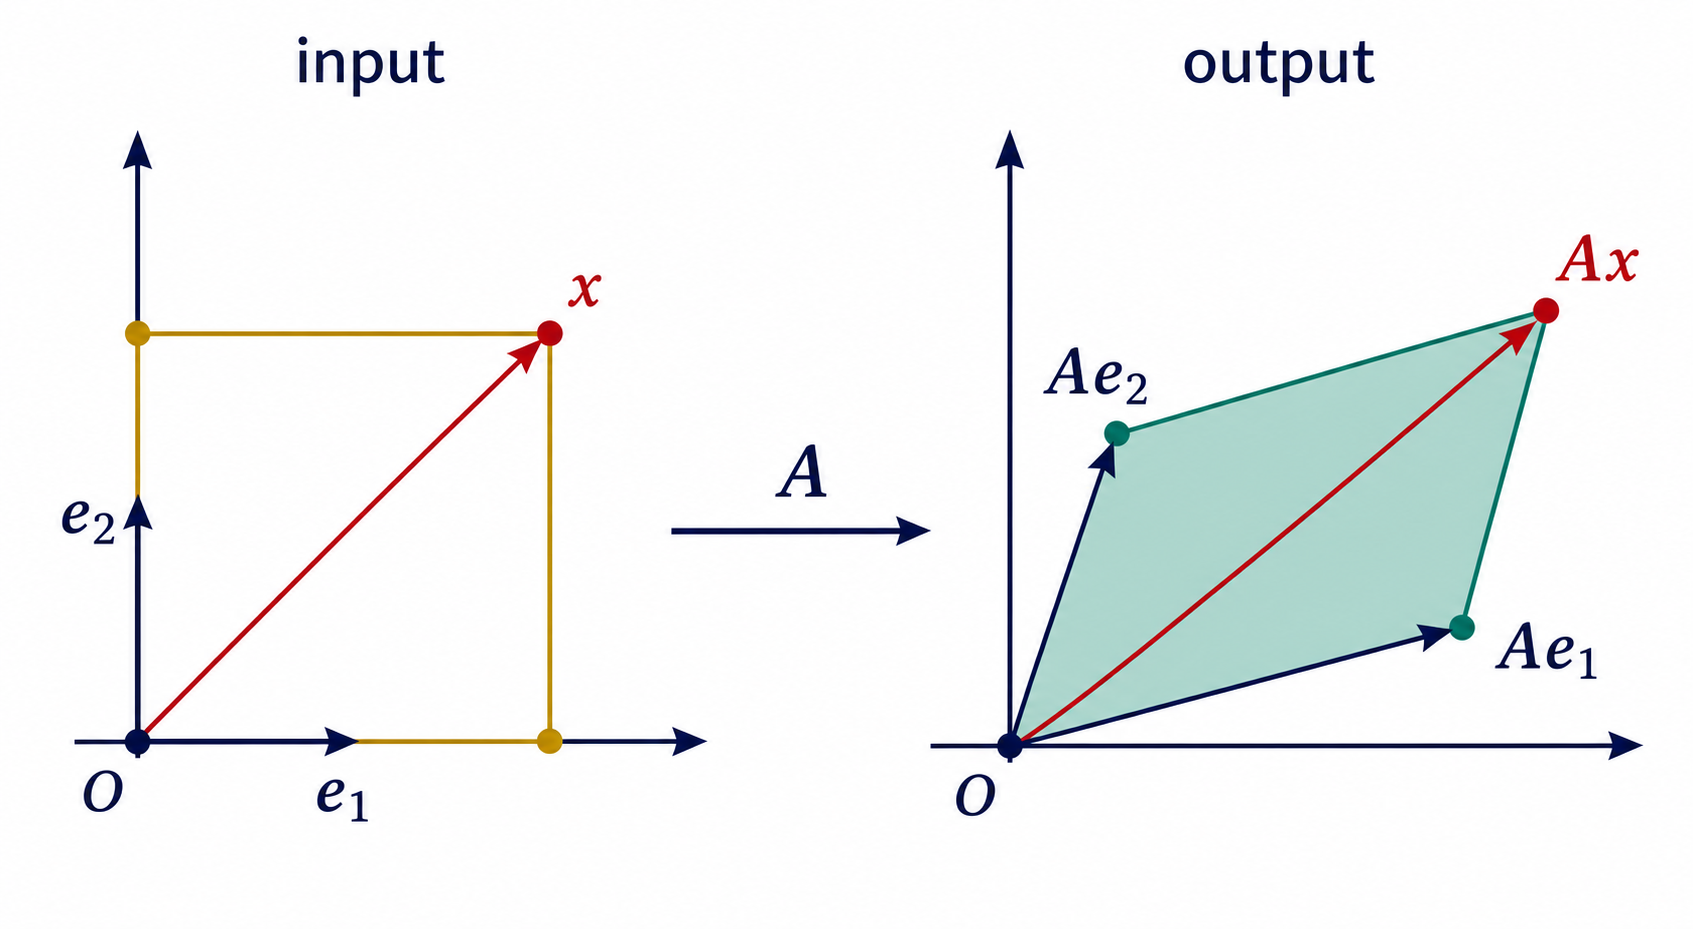
\includegraphics[width=0.95\linewidth]{imagegen-figures/ch04-matrix-transforms-grid.png}
\caption{A matrix is determined by what it does to basis directions. In the input panel, \(x=e_1+e_2\) is the diagonal of the unit square. In the output panel, the square becomes the parallelogram spanned by \(Ae_1\) and \(Ae_2\), and the same linear combination gives \(Ax=Ae_1+Ae_2\). The columns of the matrix are the transformed basis vectors.}
\label{fig:ch04-matrix-transforms-grid}
\end{figure}

\paragraph{Formal setup.}
Let \(A\in\mathbb{R}^{m\times n}\) have entries \(a_{ij}\), where \(i=1,\dots,m\) indexes output coordinates and \(j=1,\dots,n\) indexes input coordinates:
\[
A=
\begin{bmatrix}
a_{11} & a_{12} & \cdots & a_{1n}\\
a_{21} & a_{22} & \cdots & a_{2n}\\
\vdots & \vdots & \ddots & \vdots\\
a_{m1} & a_{m2} & \cdots & a_{mn}
\end{bmatrix}.
\]
For \(x\in\mathbb{R}^n\), the matrix-vector product \(y=Ax\in\mathbb{R}^m\) is defined by
\[
y_i=\sum_{j=1}^n a_{ij}x_j,
\qquad i=1,\dots,m.
\]
Equivalently, if \(a_j=Ae_j\in\mathbb{R}^m\) is the \(j\)th column of \(A\), then
\[
Ax=x_1a_1+\cdots+x_na_n.
\]
This column formula is the central equation of the section.

A map \(T:\mathbb{R}^n\to\mathbb{R}^m\) is \emph{linear} if, for all \(u,v\in\mathbb{R}^n\) and all scalars \(\alpha,\beta\in\mathbb{R}\),
\[
T(\alpha u+\beta v)=\alpha T(u)+\beta T(v).
\]
The domain is \(\mathbb{R}^n\), the codomain is \(\mathbb{R}^m\), and the matrix that represents \(T\) in standard coordinates has columns \(T(e_1),\dots,T(e_n)\).

\paragraph{Core intuition.}
Imagine drawing a square grid on the input plane. A linear map sends the origin to the origin, sends lines to lines or collapsed points, and sends parallelograms to parallelograms. Figure~\ref{fig:ch04-matrix-transforms-grid} shows the essential mechanism: once the basis arrows move to \(Ae_1\) and \(Ae_2\), every grid point follows by the same coordinate recipe.

There are two equally useful readings of \(Ax\). The row reading says that output coordinate \(i\) is a weighted sum of input coordinates:
\[
y_i=a_{i1}x_1+\cdots+a_{in}x_n.
\]
The column reading says that the whole output is a linear combination of output-side columns:
\[
y=x_1a_1+\cdots+x_na_n.
\]
The row view is natural when each output unit computes a measurement. The column view is natural when asking what outputs are reachable.

Common misconceptions are worth removing early. First, a matrix need not be square. A \(100\times 3\) matrix maps three input features to one hundred output coordinates. Second, a matrix is not just a data table; it becomes a linear map when we specify which vectors it acts on and how. Third, the order of dimensions matters: \(A\in\mathbb{R}^{m\times n}\) maps from \(n\) coordinates to \(m\) coordinates, not the other way around. Fourth, a translation such as \(x\mapsto Ax+b\) is not linear unless \(b=0\). It is affine, and we will use affine maps often, but the matrix part is the linear part.

This section uses Chapter 3's basis expansion \(x=\sum_j x_je_j\). It prepares rank, null space, data fitting, Jacobians, neural network layers, and linearized dynamics.

\paragraph{Main theorem: matrices and linear maps in standard coordinates.}
Every matrix \(A\in\mathbb{R}^{m\times n}\) defines a linear map \(T_A:\mathbb{R}^n\to\mathbb{R}^m\) by \(T_A(x)=Ax\). Conversely, every linear map \(T:\mathbb{R}^n\to\mathbb{R}^m\) has a unique representing matrix
\[
A=\begin{bmatrix}T(e_1) & T(e_2) & \cdots & T(e_n)\end{bmatrix}.
\]

\emph{Proof sketch.} First let \(A\) be a matrix. For vectors \(u,v\in\mathbb{R}^n\) and scalars \(\alpha,\beta\),
\[
A(\alpha u+\beta v)
=\sum_{j=1}^n(\alpha u_j+\beta v_j)a_j.
\]
Each coordinate of \(\alpha u+\beta v\) becomes the coefficient of the corresponding column \(a_j\). Distribute the coefficients:
\[
A(\alpha u+\beta v)
=\alpha\sum_{j=1}^n u_ja_j+\beta\sum_{j=1}^n v_ja_j.
\]
Recognize the two column combinations:
\[
A(\alpha u+\beta v)=\alpha Au+\beta Av.
\]
So every matrix gives a linear map.

Now let \(T\) be a linear map. Every input has the standard expansion
\[
x=x_1e_1+\cdots+x_ne_n.
\]
Linearity lets \(T\) pass through this linear combination:
\[
T(x)=x_1T(e_1)+\cdots+x_nT(e_n).
\]
If we place \(T(e_j)\) as column \(j\) of a matrix \(A\), the right-hand side is exactly \(Ax\). The matrix is unique because column \(j\) must equal \(Ae_j=T(e_j)\). A linear map has no freedom beyond where it sends the basis directions.

\paragraph{Worked examples.}
\emph{Small numerical example.} Let
\[
A=
\begin{bmatrix}
2 & -1\\
1 & 1\\
0 & 3
\end{bmatrix},
\qquad
x=\begin{bmatrix}4\\-2\end{bmatrix}.
\]
The columns are
\[
a_1=\begin{bmatrix}2\\1\\0\end{bmatrix},
\qquad
a_2=\begin{bmatrix}-1\\1\\3\end{bmatrix}.
\]
The column-combination view gives
\[
Ax=4a_1-2a_2
=
4\begin{bmatrix}2\\1\\0\end{bmatrix}
-2\begin{bmatrix}-1\\1\\3\end{bmatrix}
=
\begin{bmatrix}10\\2\\-6\end{bmatrix}.
\]
The row view gives the same output by three measurements:
\[
y_1=2(4)-(-2)=10,\quad
y_2=4+(-2)=2,\quad
y_3=3(-2)=-6.
\]

\emph{Conceptual ML/neuroscience example.} In a linear neural network layer without bias,
\[
h=Wx,
\qquad W\in\mathbb{R}^{k\times d}.
\]
The input \(x\in\mathbb{R}^d\) is an activation vector from the previous layer, and the output \(h\in\mathbb{R}^k\) is the next activation before a nonlinearity. Row \(i\) of \(W\) contains the incoming weights used by output unit \(i\). Column \(j\) of \(W\) is the output pattern produced by activating input coordinate \(j\) alone. In a neural encoding model, the same mathematics appears when \(x\) is a stimulus-feature vector and \(Wx\) predicts a population firing-rate vector.

\paragraph{ML/DL/neuroscience connections.}
In machine learning, matrices map feature vectors to scores, hidden activations, logits, and predictions. In deep learning, a dense layer is an affine map \(x\mapsto Wx+b\); the matrix \(W\) is the linear part and \(b\) shifts the output. In computational neuroscience, a linear receptive-field model maps stimulus coordinates to predicted neural responses, and a linear decoder maps population activity to an estimate of stimulus, choice, or movement. Later, Jacobian matrices will describe local linear maps of nonlinear systems, and convolutional layers will be represented as structured linear maps.

\paragraph{Exercises.}
\begin{enumerate}[label=\textbf{4.1.\arabic*.}, leftmargin=*]
\item \textbf{Mechanical.} For
\[
A=\begin{bmatrix}1&2&0\\ -1&3&4\end{bmatrix},
\qquad
x=\begin{bmatrix}2\\-1\\3\end{bmatrix},
\]
compute \(Ax\) using both the row view and the column-combination view.
\item \textbf{Proof or derivation.} Let \(A\in\mathbb{R}^{m\times n}\). Prove directly from the column formula that \(A(0)=0\) and \(A(\alpha x+\beta y)=\alpha Ax+\beta Ay\).
\item \textbf{Numerical/computational.} Write pseudocode for computing \(y=Ax\) by looping over rows. Then write pseudocode for computing the same \(y\) by adding scaled columns. State the dimensions of all arrays.
\item \textbf{Interpretation.} In a weight matrix \(W\in\mathbb{R}^{k\times d}\) for a linear layer, what does row \(i\) mean? What does column \(j\) mean?
\item \textbf{Debug the misconception.} A student says, ``The matrix \(A\) has \(m\) rows and \(n\) columns, so it maps \(\mathbb{R}^m\) to \(\mathbb{R}^n\).'' Explain the dimension error and give the correct domain and codomain.
\end{enumerate}

\subsection{4.2 Composition, inverses, and change of basis}

\paragraph{Motivating question.}
If we apply linear maps in sequence, undo a linear map, or describe the same map in different coordinates, how should the matrices change?

\paragraph{Beginner setup.}
Three operations organize matrix algebra.

\emph{Composition} means doing one linear map after another. If \(B\) sends \(x\) to \(Bx\), and then \(A\) sends that result to \(A(Bx)\), the combined matrix is \(AB\).

\emph{Inversion} means undoing a map exactly. A square matrix \(A\in\mathbb{R}^{n\times n}\) is invertible if there is a matrix \(A^{-1}\) with
\[
A^{-1}A=I_n
\qquad\text{and}\qquad
AA^{-1}=I_n.
\]
Not every square matrix is invertible. A map that collapses two different inputs to the same output cannot be undone.
Equivalently, an invertible linear map must preserve enough information to distinguish inputs and must reach every output in its codomain. In the language of Section 4.3, this will mean no nonzero null-space direction and full rank.

\emph{Change of basis} means re-expressing the same geometric map using different coordinate systems. The vector has not changed; only the numbers used to describe it have changed.

The smallest nontrivial composition example uses two \(2\times 2\) matrices. If
\[
B=
\begin{bmatrix}
1&1\\
0&1
\end{bmatrix}
\quad\text{and}\quad
A=
\begin{bmatrix}
2&0\\
0&3
\end{bmatrix},
\]
then \(B\) shears the plane and \(A\) rescales the two coordinate axes. The product \(AB\) means shear first, rescale second.

What to keep in mind: the order in \(ABx\) is read from right to left at the level of actions. The matrix next to \(x\) acts first.

\begin{figure}[htbp]
\centering
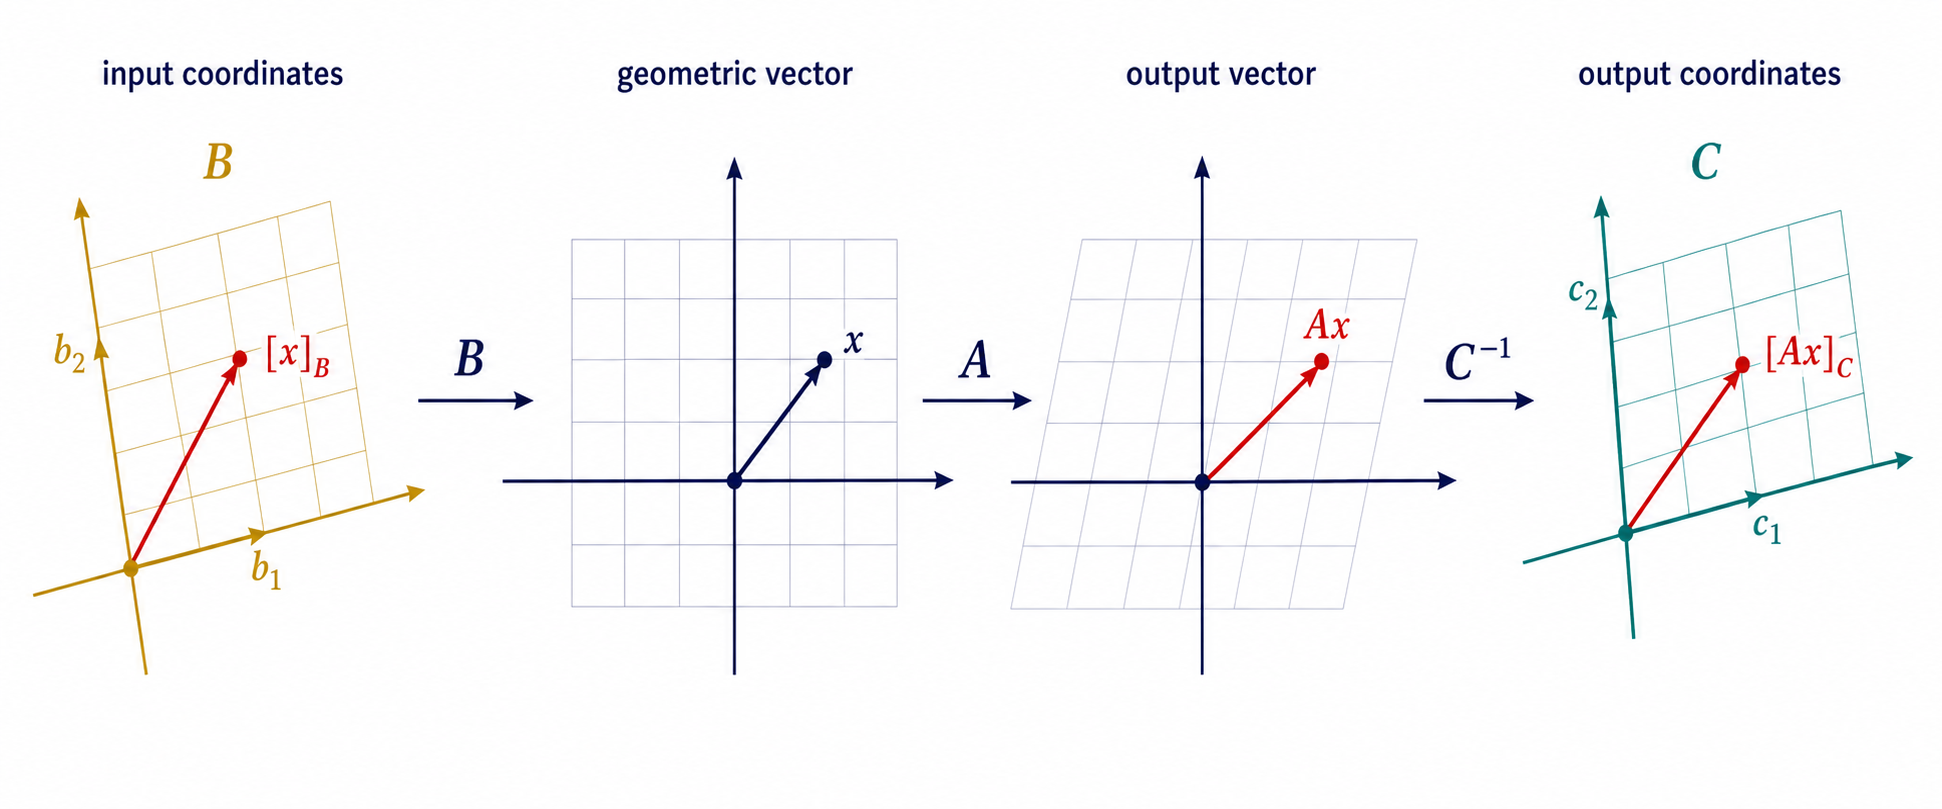
\includegraphics[width=0.98\linewidth]{imagegen-figures/ch04-composition-change-basis.png}
\caption{The change-of-basis formula is a composition. Starting with coordinates \([x]_B\), the basis matrix \(B\) reconstructs the geometric vector \(x\). The map \(A\) sends it to \(Ax\). The inverse coordinate matrix \(C^{-1}\) remeasures the output in the \(C\)-basis, producing \([Ax]_C=C^{-1}AB[x]_B\).}
\label{fig:ch04-composition-change-basis}
\end{figure}

\paragraph{Formal setup.}
Let \(S:\mathbb{R}^p\to\mathbb{R}^n\) have matrix \(B\in\mathbb{R}^{n\times p}\), and let \(T:\mathbb{R}^n\to\mathbb{R}^m\) have matrix \(A\in\mathbb{R}^{m\times n}\). The composition \(T\circ S:\mathbb{R}^p\to\mathbb{R}^m\) has matrix \(AB\in\mathbb{R}^{m\times p}\):
\[
(T\circ S)(x)=T(S(x))=A(Bx)=(AB)x.
\]
The entry formula for the product is
\[
(AB)_{ik}=\sum_{j=1}^n a_{ij}b_{jk}.
\]
Here \(j\) indexes the intermediate coordinate that is produced by \(B\) and consumed by \(A\).

For inversion, \(A\in\mathbb{R}^{n\times n}\) is invertible if there exists \(A^{-1}\in\mathbb{R}^{n\times n}\) satisfying
\[
A^{-1}A=AA^{-1}=I_n.
\]
This algebraic identity means the linear map \(x\mapsto Ax\) is both one-to-one and onto: \(Ax=Ay\) forces \(x=y\), and every output \(b\in\mathbb{R}^n\) has a unique input \(x=A^{-1}b\). For rectangular matrices the two ideas separate: a tall matrix may distinguish inputs without reaching every output, while a wide matrix may reach many outputs but still have nonunique inputs.

For change of basis, let \(T:\mathbb{R}^n\to\mathbb{R}^m\) have standard matrix \(A\). Let \(B\in\mathbb{R}^{n\times n}\) be an input basis matrix, whose columns are the input basis vectors, and let \(C\in\mathbb{R}^{m\times m}\) be an output basis matrix. If \([x]_B\) is the input coordinate vector and \([T(x)]_C\) is the output coordinate vector, then
\[
[T]_B^C=C^{-1}AB,
\qquad
[T(x)]_C=C^{-1}AB[x]_B.
\]
When the same basis \(P\) is used for both input and output of a map \(\mathbb{R}^n\to\mathbb{R}^n\), this becomes the similarity transformation
\[
[T]_P=P^{-1}AP.
\]

\paragraph{Core intuition.}
Composition is function composition written in coordinates. The product \(AB\) stores all paths that go from an input coordinate, through an intermediate coordinate, to an output coordinate. The sum \(\sum_j a_{ij}b_{jk}\) collects every intermediate route from input \(k\) to output \(i\).

An inverse exists only when the map loses no information. If a matrix squashes the plane onto a line, many inputs share one output, so no rule can recover the original input from the output. If the map stretches, rotates, or shears without collapse, an inverse map can undo it.

Change of basis is often the most conceptually confusing because it mixes objects and coordinates. Figure~\ref{fig:ch04-composition-change-basis} gives the safe reading:
\[
\text{coordinates} \xrightarrow{\;B\;} \text{vector}
\xrightarrow{\;A\;} \text{mapped vector}
\xrightarrow{\;C^{-1}\;} \text{new coordinates}.
\]
The formula \(C^{-1}AB\) is not a trick. It says reconstruct, transform, remeasure.

Common misconceptions: \(AB\) and \(BA\) are usually different because the action order changes. \(A^{-1}\) is not formed by taking reciprocals of entries. A change of basis does not change the underlying linear map; it changes its coordinate description. Finally, \(P^{-1}AP\) is not a new dynamical system if it is only a coordinate change; it is the same system described in a different basis.

This section extends Chapter 2's coordinate systems and Chapter 3's basis language. It prepares eigenvectors, diagonalization, recurrent linear dynamics, normalizing transformations, and the layer-by-layer composition of neural networks.

\paragraph{Main derivation: product and change-of-basis formulas.}
For composition, let \(x\in\mathbb{R}^p\). First \(B\) forms the intermediate vector \(z=Bx\), whose coordinate \(j\) is
\[
z_j=\sum_{k=1}^p b_{jk}x_k.
\]
Then \(A\) forms \(y=Az\), whose coordinate \(i\) is
\[
y_i=\sum_{j=1}^n a_{ij}z_j.
\]
Substitute the expression for \(z_j\):
\[
y_i=\sum_{j=1}^n a_{ij}\left(\sum_{k=1}^p b_{jk}x_k\right).
\]
Regroup the terms by input coordinate \(x_k\):
\[
y_i=\sum_{k=1}^p\left(\sum_{j=1}^n a_{ij}b_{jk}\right)x_k.
\]
Therefore the coefficient from input \(k\) to output \(i\) is
\[
(AB)_{ik}=\sum_{j=1}^n a_{ij}b_{jk}.
\]
The inner sum is over the intermediate coordinate, exactly matching the idea of a two-stage map.

For change of basis, start with input coordinates \([x]_B\). Reconstruct the actual vector:
\[
x=B[x]_B.
\]
Apply the standard matrix \(A\):
\[
T(x)=A B[x]_B.
\]
Remeasure the output in the \(C\)-basis. Since \(v=C[v]_C\), we have \([v]_C=C^{-1}v\), so
\[
[T(x)]_C=C^{-1}AB[x]_B.
\]
Thus the matrix that takes \(B\)-coordinates of the input directly to \(C\)-coordinates of the output is \(C^{-1}AB\).

\paragraph{Worked examples.}
\emph{Small numerical example.} Let
\[
A=\begin{bmatrix}2&0\\0&3\end{bmatrix},
\qquad
B=\begin{bmatrix}1&1\\0&1\end{bmatrix}.
\]
Then
\[
AB=
\begin{bmatrix}2&2\\0&3\end{bmatrix},
\qquad
BA=
\begin{bmatrix}2&3\\0&3\end{bmatrix}.
\]
The products are different. In \(ABx\), the shear \(B\) acts first and the scaling \(A\) acts second. In \(BAx\), the scaling acts first and the shear acts second. Matrix multiplication records ordered computation, not just pairwise arithmetic.

The shear is invertible:
\[
B^{-1}=
\begin{bmatrix}1&-1\\0&1\end{bmatrix},
\qquad
B^{-1}B=BB^{-1}=I_2.
\]
Geometrically, \(B\) adds the second coordinate into the first; \(B^{-1}\) subtracts it back out. No direction is collapsed.

For a change of basis example, let
\[
A=\begin{bmatrix}1&2\\0&1\end{bmatrix},
\qquad
B=
\begin{bmatrix}1&1\\0&1\end{bmatrix},
\qquad
C=I_2.
\]
Then the matrix from \(B\)-coordinates of the input to standard output coordinates is
\[
C^{-1}AB=AB
=
\begin{bmatrix}1&3\\0&1\end{bmatrix}.
\]
This does not mean the map changed. It means that the input vector is first reconstructed from the tilted \(B\)-coordinate grid and only then transformed by \(A\).

\emph{Conceptual ML/neuroscience example.} If two neural network layers are linear and have no nonlinearity or bias between them,
\[
h=W_1x,\qquad y=W_2h,
\]
then
\[
y=W_2W_1x.
\]
The two layers collapse to one linear map. Nonlinearities matter because they prevent this collapse.

In neural dynamics, suppose a latent state evolves by \(z_{t+1}=Az_t\). If a scientist re-expresses the same state in a new basis \(z=P\tilde z\), then
\[
\tilde z_{t+1}=P^{-1}AP\tilde z_t.
\]
The matrix entries change, but the underlying trajectories are the same geometric trajectories written in different coordinates.

\paragraph{ML/DL/neuroscience connections.}
Deep networks are compositions of maps. Linear pieces compose by matrix multiplication; nonlinearities, normalization, attention, and gating are inserted between those linear maps. In representation learning, changing basis corresponds to choosing different coordinates for the same latent states or embeddings. In neuroscience, a population state can be described in neuron coordinates, principal-component coordinates, or task-aligned coordinates. A recurrent matrix \(A\) and its similar form \(P^{-1}AP\) describe the same linear dynamics under different coordinates, which is why eigenvectors and modes become useful in later chapters.

\paragraph{Exercises.}
\begin{enumerate}[label=\textbf{4.2.\arabic*.}, leftmargin=*]
\item \textbf{Mechanical.} For
\[
A=\begin{bmatrix}1&2\\3&4\end{bmatrix},
\qquad
B=\begin{bmatrix}0&1\\1&0\end{bmatrix},
\]
compute \(AB\), \(BA\), and \(A(Bx)\) for \(x=(5,6)\).
\item \textbf{Proof or derivation.} Prove that if \(A\) and \(B\) are invertible \(n\times n\) matrices, then \(AB\) is invertible and \((AB)^{-1}=B^{-1}A^{-1}\). Explain why the order reverses.
\item \textbf{Numerical/computational.} Given a standard matrix \(A\) and a basis matrix \(P\), write pseudocode to compute the coordinate matrix \(P^{-1}AP\) without explicitly forming \(P^{-1}\). Hint: solve \(PX=AP\) for \(X\).
\item \textbf{Interpretation.} In a recurrent neural system \(z_{t+1}=Az_t\), what changes and what stays invariant when we replace \(z_t=P\tilde z_t\)?
\item \textbf{Debug the misconception.} A student says, ``Since \(AB\) and \(BA\) use the same two matrices, they must represent the same transformation.'' Give a concrete reason this is false.
\end{enumerate}

\subsection{4.3 Rank, null space, and column space}

\paragraph{Motivating question.}
Which input directions can a matrix not see, which outputs can it actually produce, and how many independent directions survive the map?

\paragraph{Beginner setup.}
Three subspaces describe what a matrix preserves and what it loses.

The \emph{column space} of \(A\), written \(\operatorname{Col}(A)\), is the set of all outputs \(Ax\). It is the reachable part of the codomain.

The \emph{null space} of \(A\), written \(\mathcal{N}(A)\), is the set of all inputs sent to zero. It is the invisible part of the domain.

The \emph{rank} of \(A\) is the dimension of the column space. It counts how many independent output directions the map can produce.

The smallest useful example is
\[
A=
\begin{bmatrix}
1&2\\
2&4
\end{bmatrix}.
\]
The second column is twice the first, so every output is a multiple of \((1,2)\). The column space is a line:
\[
\operatorname{Col}(A)=\operatorname{span}\left\{\begin{bmatrix}1\\2\end{bmatrix}\right\}.
\]
The input vector \((-2,1)\) is invisible because
\[
A\begin{bmatrix}-2\\1\end{bmatrix}
=
\begin{bmatrix}0\\0\end{bmatrix}.
\]
So \(\mathcal{N}(A)=\operatorname{span}\{(-2,1)\}\), and \(\operatorname{rank}(A)=1\).

These objects solve different problems. Column space answers solvability: can \(Ax=b\) reach this \(b\)? Null space answers identifiability: can two different inputs produce the same output? Rank answers dimensional compression: how many degrees of freedom remain after the map acts?

What to keep in mind: the null space lives in the input space \(\mathbb{R}^n\), while the column space lives in the output space \(\mathbb{R}^m\). They are not subspaces of the same ambient space unless \(m=n\), and even then they play different roles.

\begin{figure}[htbp]
\centering
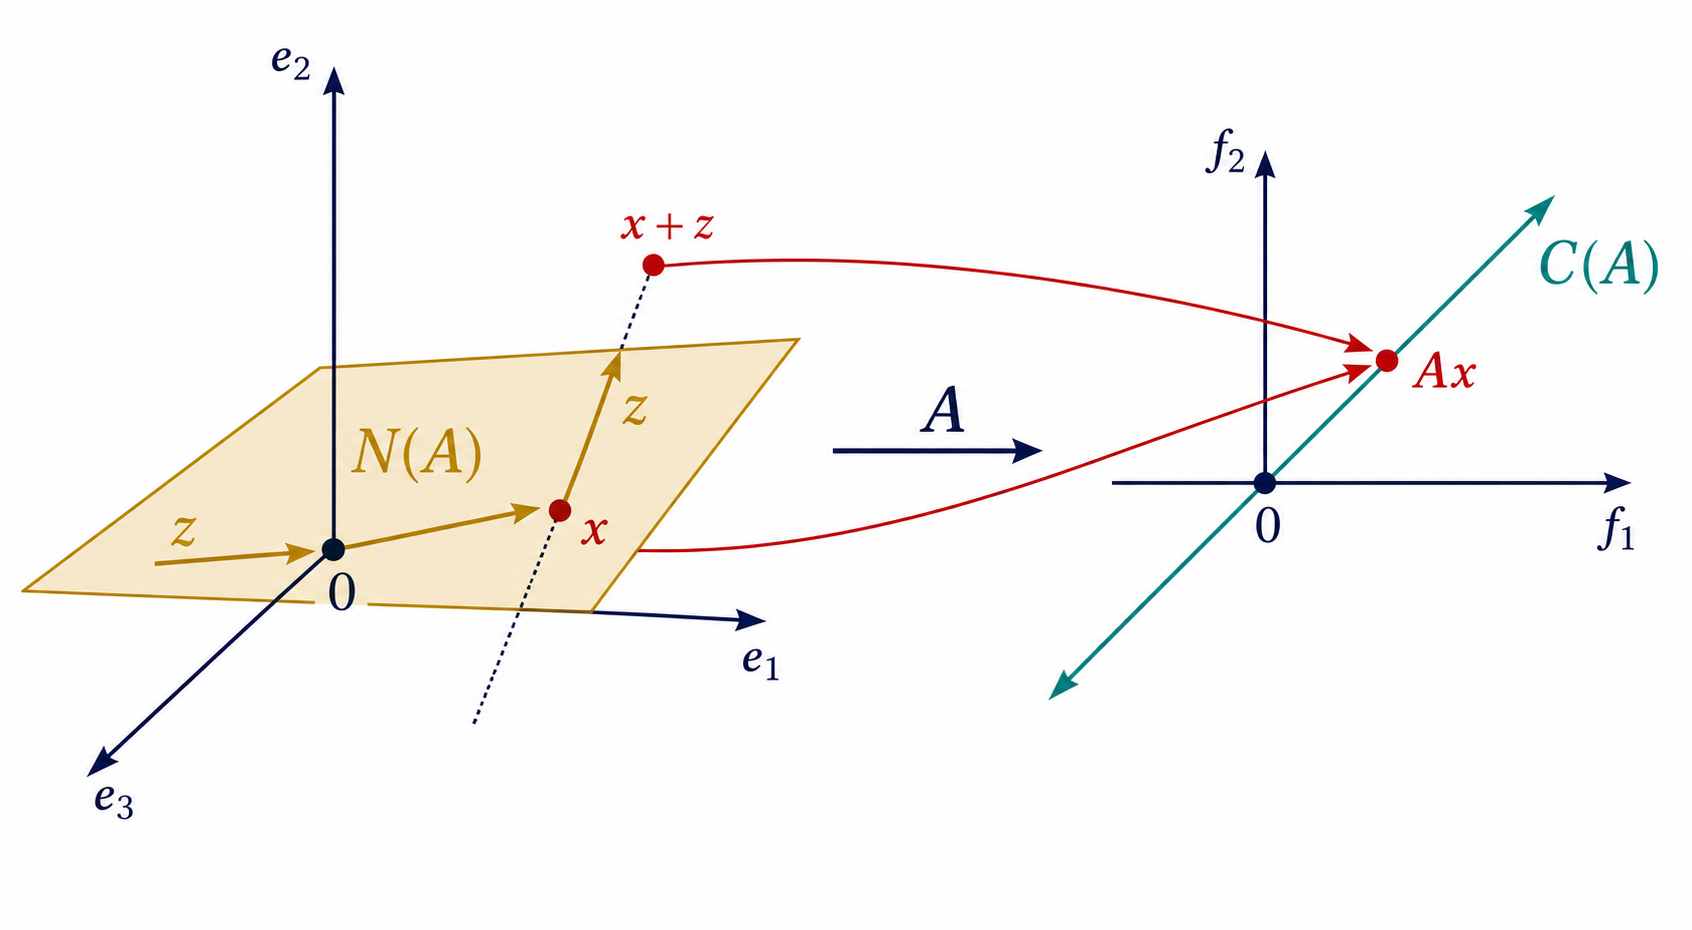
\includegraphics[width=0.95\linewidth]{imagegen-figures/ch04-rank-null-column-space.png}
\caption{Null-space directions disappear, and column-space directions are the reachable outputs. If \(z\in\mathcal{N}(A)\), then \(A(x+z)=Ax\), so all points in the same null-space fiber have the same image. The image must lie in \(\operatorname{Col}(A)\), the subspace spanned by the columns of \(A\).}
\label{fig:ch04-rank-null-column-space}
\end{figure}

\paragraph{Formal setup.}
Let \(A\in\mathbb{R}^{m\times n}\). Its column space is
\[
\operatorname{Col}(A)
=\{Ax:x\in\mathbb{R}^n\}
=\operatorname{span}\{a_1,\dots,a_n\}
\subseteq\mathbb{R}^m,
\]
where \(a_j=Ae_j\) is column \(j\). Its null space is
\[
\mathcal{N}(A)=\{x\in\mathbb{R}^n:Ax=0\}
\subseteq\mathbb{R}^n.
\]
Both are subspaces. The rank is
\[
\operatorname{rank}(A)=\dim\operatorname{Col}(A).
\]
The nullity is
\[
\operatorname{nullity}(A)=\dim\mathcal{N}(A).
\]
A linear system \(Ax=b\) is solvable exactly if and only if
\[
b\in\operatorname{Col}(A).
\]
If \(x_0\) is one solution, then every solution has the form
\[
x=x_0+z,
\qquad z\in\mathcal{N}(A),
\]
because \(A(x_0+z)=Ax_0+Az=b\).

\paragraph{Core intuition.}
The column space is the shadow or footprint of the whole input space after the matrix acts. If the columns span all of \(\mathbb{R}^m\), every output is reachable. If the columns span only a plane or line, outputs outside that subspace are impossible.

The null space is the set of directions that collapse to the origin. More generally, if \(z\in\mathcal{N}(A)\), then
\[
A(x+z)=Ax.
\]
So \(x\) and \(x+z\) are indistinguishable to the matrix. Figure~\ref{fig:ch04-rank-null-column-space} shows this as parallel input fibers mapping to the same output.

Rank counts surviving independent directions. A rank-0 map sends everything to zero. A rank-1 map produces outputs along a line. A rank-2 map produces outputs in a plane, and so on. For an \(m\times n\) matrix, the rank can never exceed \(\min(m,n)\).

Common misconceptions: rank is not the number of rows or columns; it is the number of independent output directions. A zero column does not by itself determine the rank, because other columns may span many directions. A nonzero matrix can have a nontrivial null space. Full rank means rank \(\min(m,n)\), so "full rank" means different things for tall, wide, and square matrices. Finally, a null vector is not an error; it often represents an unidentifiable parameter change or an invariance of the measurement process.

This section builds directly on Chapter 3's subspaces. It prepares least squares, PCA, singular values, identifiability in statistical models, controllability and observability, and low-dimensional neural population structure.

\paragraph{Main theorem: rank-nullity.}
For \(A\in\mathbb{R}^{m\times n}\),
\[
\operatorname{rank}(A)+\operatorname{nullity}(A)=n.
\]
The number of input dimensions equals the number of independent directions that survive plus the number of independent directions that disappear.

\emph{Proof sketch.} Let \(r=\operatorname{nullity}(A)\), and choose a basis
\[
z_1,\dots,z_r
\]
for \(\mathcal{N}(A)\). Extend this list to a basis of the whole domain \(\mathbb{R}^n\):
\[
z_1,\dots,z_r,v_1,\dots,v_s,
\qquad r+s=n.
\]
The vectors \(z_i\) are invisible because \(Az_i=0\). The claim is that
\[
Av_1,\dots,Av_s
\]
form a basis for the column space.

First, they span the column space. Any input \(x\in\mathbb{R}^n\) can be written in the extended basis:
\[
x=\sum_{i=1}^r \alpha_i z_i+\sum_{j=1}^s \beta_j v_j.
\]
Apply \(A\):
\[
Ax=\sum_{i=1}^r \alpha_iAz_i+\sum_{j=1}^s \beta_jAv_j.
\]
The null-space terms vanish:
\[
Ax=\sum_{j=1}^s \beta_jAv_j.
\]
So every output is a combination of the \(Av_j\).

Second, the \(Av_j\) are independent. Suppose
\[
\sum_{j=1}^s \beta_jAv_j=0.
\]
By linearity,
\[
A\left(\sum_{j=1}^s \beta_jv_j\right)=0.
\]
Thus \(\sum_j\beta_jv_j\in\mathcal{N}(A)\). Since \(z_1,\dots,z_r\) are a basis of the null space, this vector can also be written as a combination of the \(z_i\). But the full list \(z_1,\dots,z_r,v_1,\dots,v_s\) is independent, so all \(\beta_j=0\). Therefore \(Av_1,\dots,Av_s\) are independent.

There are \(s=n-r\) basis vectors for the column space, so
\[
\operatorname{rank}(A)=s=n-r.
\]
Rearranging gives \(\operatorname{rank}(A)+\operatorname{nullity}(A)=n\).

\paragraph{Worked examples.}
\emph{Small numerical example.} Let
\[
A=
\begin{bmatrix}
1&2&0\\
0&1&1\\
1&3&1
\end{bmatrix}.
\]
The columns are
\[
c_1=\begin{bmatrix}1\\0\\1\end{bmatrix},
\qquad
c_2=\begin{bmatrix}2\\1\\3\end{bmatrix},
\qquad
c_3=\begin{bmatrix}0\\1\\1\end{bmatrix}.
\]
Since \(c_2=2c_1+c_3\), the columns are dependent. Since \(c_1\) and \(c_3\) are not scalar multiples, they are independent. Therefore
\[
\operatorname{Col}(A)=\operatorname{span}\{c_1,c_3\},
\qquad
\operatorname{rank}(A)=2.
\]
To find the null space, solve \(Ax=0\):
\[
x_1+2x_2=0,
\qquad
x_2+x_3=0.
\]
Let \(x_2=t\). Then \(x_1=-2t\) and \(x_3=-t\), so
\[
\mathcal{N}(A)=\operatorname{span}\left\{
\begin{bmatrix}-2\\1\\-1\end{bmatrix}
\right\}.
\]
The nullity is \(1\). Rank-nullity checks:
\[
2+1=3,
\]
which equals the input dimension.

\emph{Conceptual ML/neuroscience example.} In linear regression, a design matrix \(X\in\mathbb{R}^{n\times d}\) maps a parameter vector \(w\in\mathbb{R}^d\) to predictions \(Xw\in\mathbb{R}^n\). If \(z\in\mathcal{N}(X)\), then \(X(w+z)=Xw\). The parameter change \(z\) is unidentifiable from the data because it changes the weights but not the predictions. In neuroscience, if a decoder matrix maps population activity \(r\) to an estimated variable \(Dr\), then \(\mathcal{N}(D)\) consists of population activity changes that the decoder ignores, while \(\operatorname{Col}(D)\) is the space of estimates the decoder can produce.

\paragraph{ML/DL/neuroscience connections.}
Rank measures effective linear dimensionality. In ML, rank-deficient design matrices create non-unique fitted parameters. In deep learning, low-rank weight matrices constrain information flow through a layer and motivate low-rank adaptation methods. In neuroscience, a neural population may have many recorded neurons but only a smaller number of task-relevant activity directions; linear decoders expose which directions are read out and which directions lie in a decoder null space. Later, singular values will quantify not only how many directions survive, but how strongly each direction is amplified or suppressed.

\paragraph{Exercises.}
\begin{enumerate}[label=\textbf{4.3.\arabic*.}, leftmargin=*]
\item \textbf{Mechanical.} For
\[
A=\begin{bmatrix}1&0&2\\0&1&-1\end{bmatrix},
\]
find \(\operatorname{Col}(A)\), \(\mathcal{N}(A)\), \(\operatorname{rank}(A)\), and \(\operatorname{nullity}(A)\).
\item \textbf{Proof or derivation.} Prove that \(\mathcal{N}(A)\) is a subspace of \(\mathbb{R}^n\) and that \(\operatorname{Col}(A)\) is a subspace of \(\mathbb{R}^m\).
\item \textbf{Numerical/computational.} Write pseudocode that computes \(\operatorname{rank}(A)\) by scanning the columns of \(A\), keeping a list of independent columns, and testing whether each new column lies in the span of the columns already kept. What should the algorithm return when all columns are combinations of earlier kept columns?
\item \textbf{Interpretation.} If a decoder \(D\) has a large null space, what kinds of neural population changes are invisible to the decoded output?
\item \textbf{Debug the misconception.} A student says, ``Since \(A\) has three columns, its rank is three.'' Give a counterexample and state the correct criterion.
\end{enumerate}

\subsection{4.4 Linear systems and data fitting}

\paragraph{Motivating question.}
When can the equations \(Ax=b\) be solved exactly, and what should we do when noisy data make exact solution impossible?

\paragraph{Beginner setup.}
A \emph{linear system} is an equation
\[
Ax=b,
\]
where \(A\in\mathbb{R}^{m\times n}\) is known, \(b\in\mathbb{R}^m\) is known, and \(x\in\mathbb{R}^n\) is unknown. Each row of \(A\) gives one linear equation. Each column of \(A\) gives one direction in output space that can be combined to reach \(b\).

Exact solution is possible precisely when \(b\) lies in the column space of \(A\). If \(b\notin\operatorname{Col}(A)\), no choice of \(x\) can make \(Ax=b\). In data problems this is normal: measurements are noisy, models are simplified, and there may be more equations than unknowns.

The smallest inconsistent example is
\[
\begin{bmatrix}1\\1\end{bmatrix}x
=
\begin{bmatrix}1\\2\end{bmatrix}.
\]
It asks for one number \(x\) that equals both \(1\) and \(2\). No exact solution exists. The best least-squares choice is \(x=1.5\), which makes the fitted vector
\[
\begin{bmatrix}1.5\\1.5\end{bmatrix}
\]
as close as possible to \((1,2)\) along the reachable line \(\operatorname{Col}(A)=\operatorname{span}\{(1,1)\}\).

Linear systems solve the problem of matching constraints. Least squares solves the relaxed problem of fitting the closest reachable vector when the constraints cannot all be satisfied.

What to keep in mind: the unknown \(x\) lives in parameter/input space, while the residual \(b-Ax\) lives in output/data space. Confusing these two spaces is a common source of errors.

\begin{figure}[htbp]
\centering
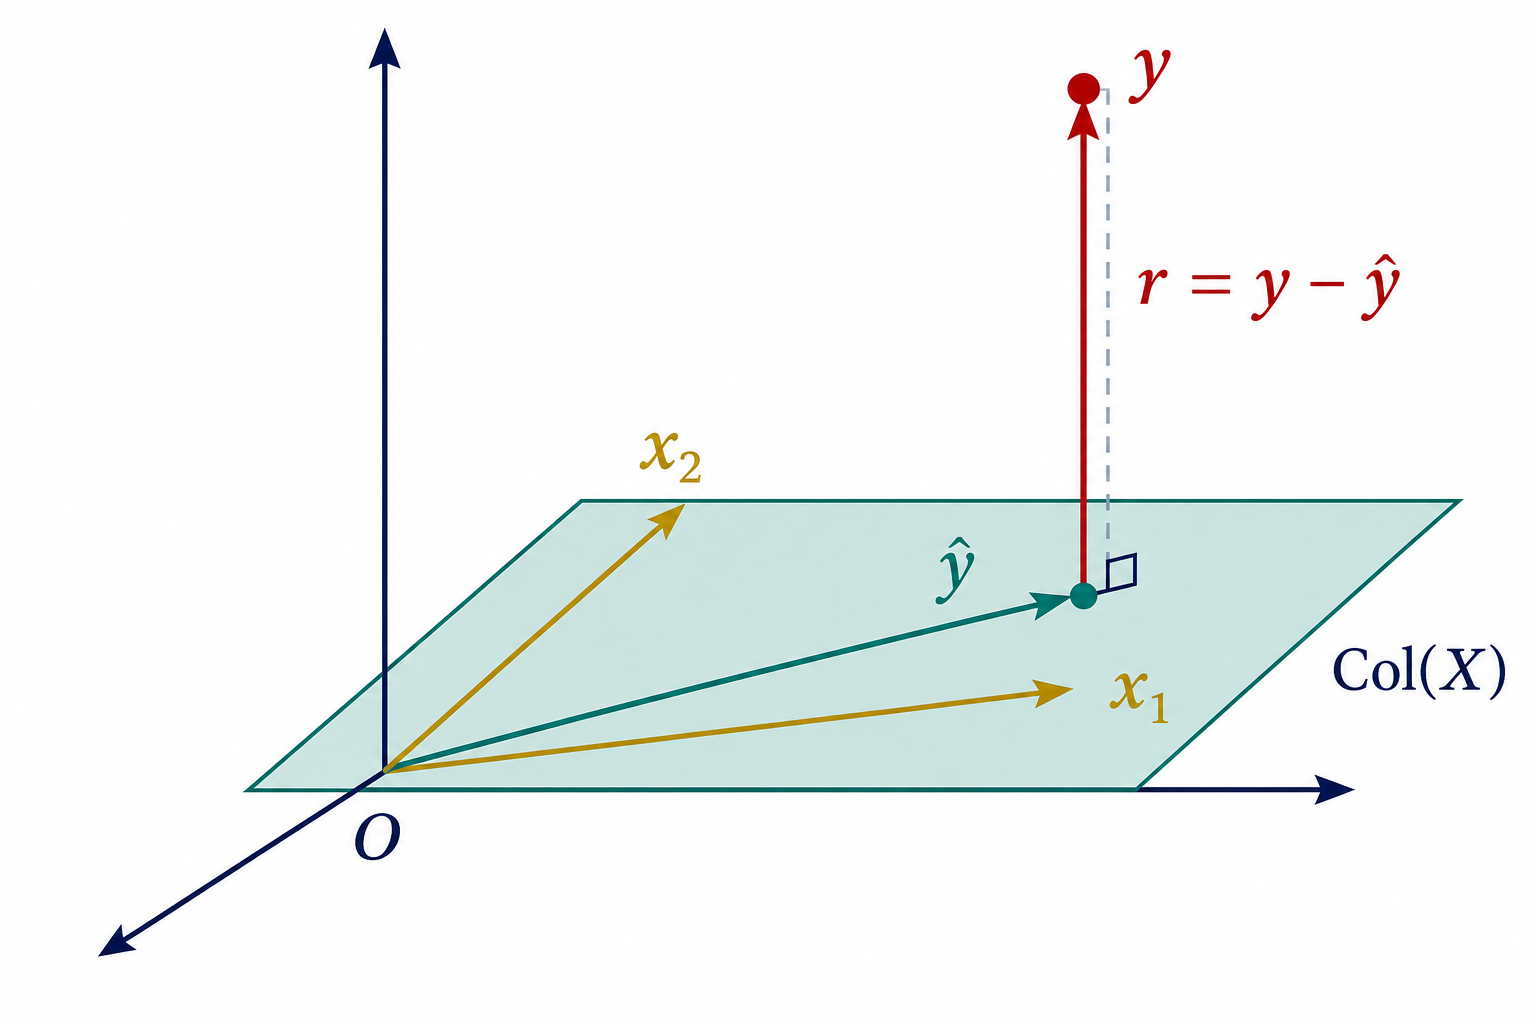
\includegraphics[width=0.90\linewidth]{imagegen-figures/ch04-linear-systems-fitting.png}
\caption{An inconsistent system becomes a closest-fit problem. The model can only produce vectors in \(\operatorname{Col}(X)\). The target \(y\) lies outside that plane, so least squares chooses the reachable vector \(\hat y=X\hat w\) closest to \(y\). The residual \(r=y-\hat y\) is perpendicular to the column space, which gives the normal equations \(X^\top r=0\).}
\label{fig:ch04-linear-systems-fitting}
\end{figure}

\paragraph{Formal setup.}
Let \(A\in\mathbb{R}^{m\times n}\), \(b\in\mathbb{R}^m\), and unknown \(x\in\mathbb{R}^n\). The exact system
\[
Ax=b
\]
has a solution if and only if \(b\in\operatorname{Col}(A)\). If \(x_0\) is one exact solution, all exact solutions are
\[
x_0+\mathcal{N}(A)=\{x_0+z:z\in\mathcal{N}(A)\}.
\]

When \(m>n\), the system is \emph{tall}: there are more equations than unknowns, so exact consistency is a special condition on \(b\). When \(m<n\), the system is \emph{wide}: there are fewer equations than unknowns, so exact solutions, if they exist, are usually nonunique because null-space directions can be added. Square systems \(m=n\) have a unique solution for every \(b\) exactly when \(A\) is invertible.

When exact solution is impossible or undesirable, the least-squares problem is
\[
\hat x\in\arg\min_{x\in\mathbb{R}^n}\|Ax-b\|_2^2.
\]
The fitted output is
\[
\hat b=A\hat x\in\operatorname{Col}(A),
\]
and the residual is
\[
r=b-\hat b=b-A\hat x.
\]
At a least-squares solution, the residual is orthogonal to every column of \(A\):
\[
A^\top r=0.
\]
Equivalently,
\[
A^\top A\hat x=A^\top b.
\]
These are the \emph{normal equations}. If the columns of \(A\) are independent, then \(A^\top A\) is invertible and
\[
\hat x=(A^\top A)^{-1}A^\top b.
\]

\paragraph{Core intuition.}
The column space is the set of all model predictions. Solving \(Ax=b\) asks whether the target \(b\) is reachable. Least squares asks for the reachable point closest to \(b\). Figure~\ref{fig:ch04-linear-systems-fitting} shows the geometric picture: drop \(b\) perpendicularly onto the column space. The foot of that perpendicular is \(\hat b=A\hat x\). The leftover vector \(r=b-\hat b\) is not random algebraic debris; it is the part of the data vector not explained by the model subspace.

The orthogonality condition \(A^\top r=0\) has a direct meaning. Each column \(a_j\) of \(A\) is a direction in which the fitted vector could move by changing parameter \(x_j\). If the residual had a component along any column, moving a little in that direction would reduce the error. At the best fit, no column direction can reduce the residual further.

Common misconceptions: least squares does not make every equation equally accurate; it minimizes the sum of squared residuals. The formula \((A^\top A)^{-1}A^\top b\) is valid only when \(A\) has independent columns. Solving normal equations can be numerically less stable than QR or SVD methods, which will appear later. Finally, a small residual does not prove the model is scientifically correct; it only says the target is close to the model's column space under the chosen norm.

This section ties Chapter 4 to Chapter 5. Here we state the fitting principle and derive the normal equations. Next, projections and least squares will be studied as geometric objects in their own right.

\paragraph{Main derivation: the normal equations.}
Let
\[
f(x)=\|Ax-b\|_2^2.
\]
Suppose \(\hat x\) minimizes \(f\), and write
\[
\hat b=A\hat x,
\qquad
r=b-\hat b.
\]
Take any direction \(z\in\mathbb{R}^n\). Changing the parameter from \(\hat x\) to \(\hat x+tz\) changes the fitted output from \(\hat b\) to \(\hat b+tAz\). The squared error as a function of \(t\) is
\[
\phi(t)=\|A(\hat x+tz)-b\|_2^2
=\|\hat b+tAz-b\|_2^2.
\]
Since \(r=b-\hat b\), this is
\[
\phi(t)=\|tAz-r\|_2^2.
\]
Expand the squared norm:
\[
\phi(t)=\|r\|_2^2-2t(Az)^\top r+t^2\|Az\|_2^2.
\]
Because \(t=0\) is a minimum for every direction \(z\), the linear term must vanish:
\[
(Az)^\top r=0
\qquad\text{for every }z.
\]
Rewrite the left side:
\[
(Az)^\top r=z^\top A^\top r.
\]
If \(z^\top A^\top r=0\) for every \(z\), then \(A^\top r=0\). Substitute \(r=b-A\hat x\):
\[
A^\top(b-A\hat x)=0.
\]
Rearranging gives the normal equations
\[
A^\top A\hat x=A^\top b.
\]
The mechanism is geometric: the residual must be perpendicular to every direction in the column space.

\paragraph{Worked examples.}
\emph{Small numerical example.} Fit a line \(y\approx \beta_0+\beta_1t\) to three points \((0,1)\), \((1,2)\), and \((2,2)\). The design matrix and target are
\[
A=
\begin{bmatrix}
1&0\\
1&1\\
1&2
\end{bmatrix},
\qquad
b=
\begin{bmatrix}
1\\2\\2
\end{bmatrix}.
\]
Compute
\[
A^\top A=
\begin{bmatrix}
3&3\\
3&5
\end{bmatrix},
\qquad
A^\top b=
\begin{bmatrix}
5\\6
\end{bmatrix}.
\]
The normal equations are
\[
\begin{bmatrix}
3&3\\
3&5
\end{bmatrix}
\begin{bmatrix}\hat\beta_0\\\hat\beta_1\end{bmatrix}
=
\begin{bmatrix}5\\6\end{bmatrix}.
\]
Solving gives
\[
\hat\beta_0=\frac{7}{6},
\qquad
\hat\beta_1=\frac{1}{2}.
\]
Thus
\[
\hat b=A\hat\beta
=
\begin{bmatrix}
7/6\\
5/3\\
13/6
\end{bmatrix},
\qquad
r=b-\hat b
=
\begin{bmatrix}
-1/6\\
1/3\\
-1/6
\end{bmatrix}.
\]
Check orthogonality:
\[
A^\top r=
\begin{bmatrix}
(-1/6)+(1/3)+(-1/6)\\
0(-1/6)+1(1/3)+2(-1/6)
\end{bmatrix}
=
\begin{bmatrix}0\\0\end{bmatrix}.
\]

\emph{Conceptual ML/neuroscience example.} In a neural encoding model, rows of \(A\) can represent trials and columns can represent stimulus features such as contrast, motion energy, or recent stimulus history. The target \(b\) is a vector of spike counts for one neuron across trials. The parameter vector \(x\) contains the neuron's feature weights. The fitted vector \(A\hat x\) is the model-predicted response across trials, and the residual \(b-A\hat x\) is the trial-by-trial activity left unexplained by the linear feature model. For a linear readout, \(A\) might instead be a matrix of neural population activity and \(b\) a behavioral variable; least squares fits decoder weights.

\paragraph{ML/DL/neuroscience connections.}
Least squares is the prototype for supervised learning. Inputs become rows of a design matrix, parameters become the unknown vector, predictions become \(Ax\), and training minimizes a loss. In deep learning, the model is nonlinear in general, but the final linear readout and many local approximations still use this geometry. In neuroscience, linear regression, encoding models, decoding models, and peri-stimulus response summaries all rely on the distinction between the reachable prediction subspace and the unexplained residual. Later chapters will generalize this picture to regularized regression, generalized linear models, probabilistic noise models, and gradient-based optimization.

\paragraph{Exercises.}
\begin{enumerate}[label=\textbf{4.4.\arabic*.}, leftmargin=*]
\item \textbf{Mechanical.} Determine whether
\[
\begin{bmatrix}
1&0\\
0&1\\
1&1
\end{bmatrix}
x
=
\begin{bmatrix}
2\\3\\5
\end{bmatrix}
\]
has an exact solution. Then determine whether the same matrix can exactly reach \(b=(2,3,6)\).
\item \textbf{Proof or derivation.} Starting from \(r=b-A\hat x\), prove that \(A^\top r=0\) is equivalent to saying that \(r\) is orthogonal to every column of \(A\).
\item \textbf{Numerical/computational.} Write pseudocode for solving a least-squares problem using the normal equations. Before using the formula \((A^\top A)^{-1}A^\top b\), include a check that the columns of \(A\) are independent; if they are not, explain why this inverse formula is not justified.
\item \textbf{Interpretation.} In a linear neural encoding model, what does a large residual vector mean? Give one mathematical interpretation and one experimental interpretation.
\item \textbf{Debug the misconception.} A student says, ``If \(Ax=b\) has no exact solution, linear algebra has failed.'' Explain why least squares is still a linear-algebraic solution strategy and what problem it solves instead.
\end{enumerate}

The main lesson of the chapter is that a matrix is a structured map, not just a table of numbers. Its columns show the reachable output directions, its rows show the measurements being made, its products encode composed transformations, and its null space records lost input directions. Chapter 5 keeps the same column-space picture but adds orthogonality: when data are not exactly reachable, the best fit is the projection onto the reachable subspace. Chapter 6 then asks which directions a matrix treats as special, leading to eigenvectors, singular values, low-rank approximation, and PCA.

\clearpage
